\documentclass[hidelinks, 12pt]{report}
\usepackage{graphicx}
\usepackage{marginnote}
\usepackage{amsmath}
\usepackage{geometry}
\usepackage[document]{ragged2e}
\usepackage[utf8]{inputenc}
\usepackage[english]{babel}
\usepackage{fancyhdr}
\usepackage{float}
%\usepackage{floatrow}
\usepackage{caption}
%\usepackage{calc}
\usepackage{chngcntr}
\usepackage[caption = false]{subfig}
\usepackage[subfigure]{tocloft}
\newlength{\mylen}
\usepackage[font=footnotesize,labelfont=bf]{caption}
%\usepackage{times}
\usepackage[table]{xcolor}
\usepackage[intoc]{nomencl}
\usepackage{setspace}
\usepackage{tocloft}

%\usepackage{nomencl}
%\let\abbrev\nomenclature
%\makenomenclature 
%\newcommand{\Abkuerzung}{
%\printnomenclature
%\newpage
}


\usepackage{array}
\usepackage{hyperref}
\hypersetup{
    colorlinks=true,
    linkcolor=blue,
    filecolor=green,      
    urlcolor=cyan,
    citecolor=magenta,
}
\urlstyle{same}
\usepackage{bookmark}
\renewcommand{\cftfigpresnum}{\figurename\enspace}
\renewcommand{\cftfigaftersnum}{:}
\settowidth{\mylen}{\cftfigaftersnum\cftfigpresnum}
\addtolength{\cftfignumwidth}{\mylen}
\counterwithin{figure}{section}

\renewcommand{\cfttabpresnum}{\tablename\enspace}
\renewcommand{\cfttabaftersnum}{:}
\settowidth{\mylen}{\cfttabaftersnum\cftfigpresnum}
\addtolength{\cfttabnumwidth}{\mylen}
\counterwithin{table}{section}

\renewcommand{\labelenumi}{(\roman{enumi})}

\geometry{margin=1in}

\usepackage{titlesec}
\titleformat{\chapter}[display]
{\normalfont %
    \Huge % %change this size to your needs for the first line
    \bfseries}{\chaptertitlename\ \thechapter}{20pt}{%
    \huge} %change this size to your needs for the second line
 


\fancyhf{}
\fancyhead[LE,LO]{\footnotesize{}}
\fancyhead[RE,RO]{\footnotesize{Free Space Optics with DWDM and Afocal Scheme}}
\fancyfoot[LE,LO]{\footnotesize{Govt. Model Engineering College}}
\fancyfoot[RE,RO]{\footnotesize\thepage}
\renewcommand{\headrulewidth}{1pt}
\renewcommand{\footrulewidth}{1pt}
%\renewcommand{\familydefault}{\rmdefault}
\newcommand{\Rnum}[1]{\uppercase\expandafter{\romannumeral#1}}
\newcommand{\rnum}[1]{\romannumeral#1\relax}
%\setcounter{secnumdepth}{4}
%\setcounter{tocdepth}{4}

\begin{document}
\pagenumbering{none}
\centering
\section*{\centering{Bonafide Certificate}}
\vspace{1cm}

\includegraphics[height=3cm,width=3cm]{logo}

\begin{center}
MODEL ENGINEERING COLLEGE\\
\vspace{0.5cm}
THRIKKAKARA, KOCHI-21\\
\vspace{0.5cm}
DEPARTMENT OF ELECTRONICS AND COMMUNICATION \\
\vspace{0.5cm}
A P J ABDUL KALAM KERALA TECHNOLOGICAL UNIVERSITY \\
\vspace{1cm}
\textit{Bonafide Certificate}
\\This is to Certify that the Seminar Report entitled\\
\vspace{0.5cm}
\textbf{A 50-m/320-Gb/s DWDM FSO Communication With Afocal Scheme} 
\\
\vspace{0.5cm}
Submitted by\\
\vspace{0.2cm}
Anjitha M\\
\vspace{0.2cm}
is a bonafide account of her work done under our supervision. \\
\end{center}

\vspace{2cm}
\begin{minipage}[t]{10cm}
\flushleft \textbf{Seminar Co-ordinator}\\
Smt. Sheeba P S\\
Assistant Professor\\
Dept. of Electronics and\\
Communication Engineering
\end{minipage}
\vspace{2cm}
\begin{minipage}[t]{5cm}
\flushleft \textbf{Seminar Guide}\\
Smt. Remya S\\
Assistant Professor\\
Dept. of Electronics and\\
Communication Engineering
\end{minipage}
%\begin{minipage}[t]{5cm}
%\flushleft Head of Department\\
%Mr. Pradeep M\\
%Associate Professor\\
%\end{minipage}

%\addcontentsline{toc}{chapter}{Abstract}
\chapter*{Abstract}
\justify
\textit{
This is a report on the paper that proposes and presents the experimental demonstration of 320-Gb/s
free-space optical (FSO) communication based on dense-wavelength-division-multiplexing
(DWDM) technology and afocal scheme. To the best of my knowledge, this is the first
one that adopts DWDM technology and afocal scheme to successfully demonstrate
50-m/320-Gb/s FSO communication. Results have shown that the free-space transmission
distance is greatly increased by the afocal scheme and that the free-space transmission
rate is significantly enhanced by the DWDM technology. DWDM FSO communication over
a 50-m free-space link with a total transmission rate of 320 Gb/s is achieved. With the aid of a low-noise amplifier and clock/data recovery at the
receiving site, good bit-error-rate (BER) performance and clear eye diagram are obtained at
a 50-m/320-Gb/s operation. Such 50-m/320-Gb/s DWDM FSO communication provides the
advantages of optical wireless communications for long transmission distance and high
transmission rate.}\\

\textit{\textbf{keyword}}- 
Afocal scheme, dense-wavelength-division multiplexing, free-space optical
communication.
%\end{keyword}
%\sep%

\pagebreak
\setcounter{page}{1}
\pagenumbering{roman}
\justify
%\onehalfspacing
\begin{spacing}{0.8}
\renewcommand{\contentsname}{Table of Contents}
\pdfbookmark{\contentsname}{Table of Contents}
\tableofcontents
\end{spacing}
\pagebreak
%line spacing
\addcontentsline{toc}{chapter}{List of Figures}
\listoffigures 
\pagebreak
\renewcommand{\nomname}{List of Abbreviations}
\addcontentsline{toc}{chapter}{List of Abbreviations}
\printnomenclature
\pagebreak
%\addcontentsline{toc}{chapter}{List of Tables}
%\listoftables
%\pagebreak

\section*{List of Abbreviations}
\begin{flushleft}
AWG - Arrayed Waveguide Grating
\vspace{0.5cm}
BER - Bit Error Rate\\
\vspace{0.5cm}
BERT - Bit Error Rate Tester\\
\vspace{0.5cm}
CDR - Clock and Data recovery\\
\vspace{0.5cm}
DWDM - Dense Wavelength Division Multiplexing \\
\vspace{0.5cm}
EDFA - erbium doped fiber amplifiers\\
\vspace{0.5cm}
FSO - Free Space Optics\\ 
\vspace{0.5cm}
Gbps - Gigabits per second\\
\vspace{0.5cm}
LED - Light Emitting Diode\\
\vspace{0.5cm}
LNA - Low Noise Amplifier\\
\vspace{0.5cm}
MZM - Mach- Zehnder Modulator \\
\vspace{0.5cm}
OFC - Optical Fiber Cable\\
\vspace{0.5cm}
OIL - Optical Interleaver\\
\vspace{0.5cm}
SMF - Single Mode Fiber\\
\vspace{0.5cm}
TOBPF - Tunable Optical Band Pass Filter\\
\vspace{0.5cm}
VOA - Variable Optical Attenuator\\
\vspace{0.5cm}
WDM - wavelength-division multiplexing\\







\end{flushleft}
\pagebreak

    

\addcontentsline{toc}{chapter}{Acknowledgement}

\section*{\centering Acknowledgement}

\justify
On the recollection of so many great favors and blessings, I offer my sincere thanks to the Almighty, the Creator and Preserver.\\
%\vspace{1cm}

I express my heartfelt gratitude to \textbf{Prof. Dr. V P Devassia}, Principal, Govt. Model Engineering College, Thrikkakara for providing me with excellent library facilities. \\
%I sincerely thank Mr. Pradeep M, Associate Professor and Head of Department of Electronics and Communication Engineering, for his timely advice and suggestions.\\

I am thankful to my seminar coordinator \textbf{Smt. Sheeba P S}, Assistant Professor, Department of Electronics and Communication Engineering for the full-fledged support and guidance. I would like to express my sincere gratitude to \textbf{Smt. Remya S}, Assistant Professor, Department of Electronics and Communication Engineering, who has always motivated me and helped me to do everything in a better way.  \\
%\vspace{1cm}

Last but not the least I am thankful to one and all of the Department of Electronics and Communication Engineering and the whole library staff for their co-operation and active involvement.
I also thank my colleagues for their support.
\hbox{} \newpage 
\pagenumbering{arabic} 
\pagestyle{fancy}
\chapter{Introduction}
\justify
At present, free-space optical (FSO) communications are being developed to create high-speed,
high security, and friendly communications employing high bandwidth and a high capacity light
signal. For a real and
practical implementation of FSO communication, long transmission distance and high transmission
rate are the major interests. In this paper, a 320-Gbps FSO communication
with afocal scheme and dense-wavelength-division-multiplexing (DWDM) technology is proposed. The free-space transmission distance is greatly increased by the afocal scheme, and
the free-space transmission rate is significantly enhanced by the DWDM technology. Afocal
scheme, which can reduce the beam size of laser beam, is expected to provide a long free space
transmission distance in an FSO communication. DWDM technology, which can fully
utilize the free-space bandwidth, is expected to enhance the transmission rate of an FSO communication. A DWDM FSO communication that utilizes different optical wavelengths to deliver
the combined data streams would be quite useful for providing higher transmission rate.
This study demonstrates a DWDM FSO communication by using an 8-wavelength system as an
example, with each wavelength carrying a data stream of 40 Gbps. A DWDM FSO communication
over a 50-m free-space link with a total transmission rate of 320 Gbps is obtained. It is the first time to successfully establish a
50 m/320 Gbps FSO communication that employs afocal scheme and DWDM technology. 
This proposed 50 m/320 Gbps DWDM FSO communication is shown to be a prominent
one and provides the advantages of optical wireless communications for long transmission
distance and high transmission rate.
\section{Optical Communication}
\subsection{Basics of Optical Communication}
\justify
Optical communication, also known as optical telecommunication, is communication at a distance using light to carry information. It can be performed visually or by using electronic devices.An optical communication system uses a transmitter, which encodes a message into an optical signal, a channel, which carries the signal to its destination, and a receiver, which reproduces the message from the received optical signal.  

\subsection{Optical Fiber Cable (OFC)}
\justify
Optical fiber is the most common type of channel for optical communications. Basically it consists of an inner glass core surrounded by a glass cladding which has a lower refractive index. Digital signals are transmitted in the form of intensity-modulated light signal which is trapped in the glass core. Light is launched into the fiber using a light source such as a Light Emitting Diode (LED) or Laser. It is detected on the other side using a photo detector such as a photo-transistor. 
The folowing figure shows the parts of an optical fiber:
\begin{figure}[H]
\centering
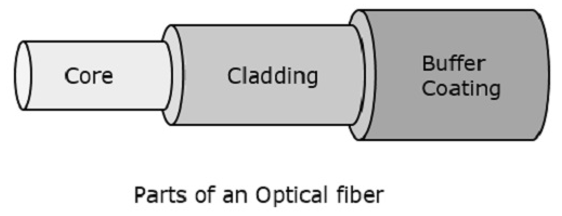
\includegraphics[width=8cm,height=4cm]{fiber_parts.jpg}
\caption[Parts of an Optical Fiber Cable]{Parts of an Optical Fiber Cable}
\label{Parts of OFC}
\end{figure}

The optical fiber cables have many advantages over the conventional co-axial cables, namely:
\begin{itemize}
  \item Higher bandwidth, therefore, can operate at higher data rates
  \item Reduced losses as signal attenuation is low.
  \item Distortion is reduced hence better quality is assured.
  \item Fiber optic cables provide high security and cannot be tapped.
  \item OFCs are immune to electromagnetic interference.
  \item These are not affected by electrical noise.
  \item Small size, light weight.
\end{itemize}
 Optical fiber transmission systems are widely used in the backbone of networks. Current optical fiber systems provide transmission rates from 45 Mb/s to 9.6 Gb/s using the single wavelength transmission.
 However, there are a few disadvantages to using OFCs, which are
 \begin{itemize}
\item The installation cost of optical fibers is higher than that for the co-axial or twisted wire cables, even though they last longer.
\item The number of repeaters are to be increased with distance.
\item They are fragile if not enclosed in a plastic sheath. Hence, more protection is needed than copper ones. 
\end{itemize}
 This is where Free Space Optics (FSO) proves to be a better choice.


\section{Free Space Optics}
\justify
Free-space optical communication (FSO) is an optical communication technology that uses light propagating in free space for wireless data transmission for telecommunications or computer networking. "Free space" means air, outer space, vacuum, or something similar. This contrasts with using solids such as optical fiber cable for data transmission.\\
\\The technology is useful where the physical connections are impractical due to high costs or other considerations. The main characteristics of free-space optical (FSO) links are high directivity, which provides
high power efficiency and isolation from other interferences, unlicensed bandwidth, easy installation,
and the promise of multi-gigabit mobile applications by using flexibility through free-space
links.\\
\\The FSO communications are attracting attention as the contemporary engineering science to resolve the last mile bottleneck issues in local area  access networks due to their high bandwidth, low cost implementation in a non-licensed spectrum, relatively low power consumption, immunity and security compared with RF technologies. 

\section{Advantages and Disadvantages of FSO}
\justify
\begin{itemize}
   \item \textbf{Advantages of FSO} 
   \begin{itemize}
     \item Ease of deployment.
    \item Can be used to power devices.
    \item License-free long-range operation (in contrast with radio communication).
    \item High bit rates.
    \item Low bit error rates.
    \item Immunity to electromagnetic interference.
    \item Full duplex operation.
    \item Protocol transparency.
    \item Increased security when working with narrow beam(s).
    \item No Fresnel zone necessary.
    \item Reference open source implementation.
     \end {itemize}
      \item \textbf{Disdvantages of FSO:}
      For terrestrial applications, there are some principal limiting factors, like:
      \begin{itemize}
      \item Fog (10 to ~100 dB/km attenuation).
    \item Beam dispersion.
    \item Atmospheric absorption.
    \item Rain.
    \item Snow.
    \item Terrestrial scintillation.
    \item Interference from background light sources (including the sun).
    \item Shadowing.
    \item Pointing stability in wind.
    \item Pollution / smog.
    \end {itemize}
          \end {itemize}
These factors cause an attenuated receiver signal and lead to higher bit error rate (BER). To overcome these issues, vendors found some solutions, like multi-beam or multi-path architectures, which use more than one sender and more than one receiver. To keep an eye-safe environment, good FSO systems have a limited laser power density and support laser classes 1 or 1M. FSO using wavelength 1550 nm system are capable of transmitting several times higher power than systems with 850 nm and are at the same time safe to the human eye (1M class). 
Laser class 1 is classified as eye-safe under all operating conditions.
Laser class 1M is classified as safe for viewing directly with the naked eye, provided no optical instruments are used.

\chapter{Literature Survey}
\justify
\section{Wavelength Division Multiplexing (WDM)}
In fiber-optic communications, wavelength-division multiplexing (WDM) is a technology which multiplexes a number of optical carrier signals onto a single optical fiber by using different wavelengths (i.e., colors) of laser light. This technique enables bidirectional communications over one strand of fiber, as well as multiplication of capacity.The following figure shows the WDM operating principle:
\begin{figure}[H]
\centering
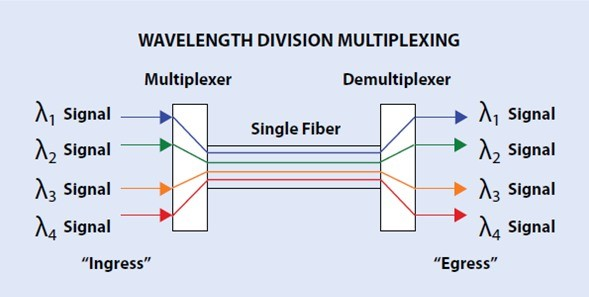
\includegraphics[width=10cm,height=8cm]{WDM-Technology-Diagram}
\caption[WDM Operating Principle]{WDM Operating Principle}
\label{WDM Operating Principle}
\end{figure}
A WDM system uses a multiplexer at the transmitter to join the several signals together, and a demultiplexer at the receiver to split them apart.\\
\\WDM systems are divided into three different wavelength patterns, \textbf{normal (WDM), coarse (CWDM) and dense (DWDM)}. Normal WDM uses the two normal wavelengths 1310 and 1550 on one fiber. Coarse WDM is defined in terms of wavelengths and provides up to 16 channels across multiple transmission windows of silica fibers. Dense wavelength division multiplexing (DWDM) is defined in terms of frequencies with denser channel spacing.  It uses wavelenghts from 1530 nm-1565 nm.
\subsection{Dense wavelength division multiplexing (DWDM)}
\justify
Dense wavelength division multiplexing (DWDM) refers originally to optical signals multiplexed within the 1550 nm band so as to leverage the capabilities (and cost) of erbium doped fiber amplifiers (EDFAs), which are effective for wavelengths between approximately 1525–1565 nm (C band), or 1570–1610 nm (L band). 
It is used to increase bandwidth over existing fiber networks.
Fig represents a general DWDM system:
\begin{figure}[H]
\centering
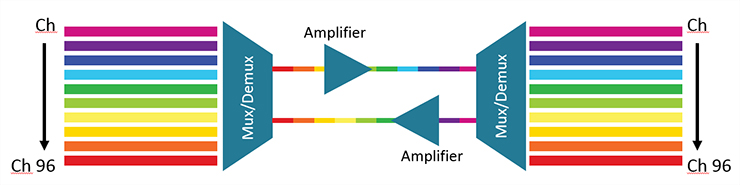
\includegraphics[width=12cm,height=4cm]{DWDM_CWDM_Connectivity.jpg}
\caption[DWDM system]{DWDM system}
\label{DWDM system}
\end{figure}
\\ 
\\DWDM works by combining and transmitting multiple signals simultaneously at different wavelengths on the same fiber. The technology creates multiple virtual fibers, thus multiplying the capacity of the physical medium.
Channel plans vary, but a typical DWDM system would use 40 channels at 100 GHz spacing or 80 channels with 50 GHz spacing. \\
\\Studies show that compared with repeater-based applications,  DWDM infrastructure also 
increases the distances between network elements,a huge benefit for long-
distance service providers looking to reduce their initial network investments 
significantly. The fiber-optic amplifier component of the DWDM system enables 
a service provider to save costs by taking in and amplifying optical signals 
without converting them to electrical signals. Furthermore, DWDM allows 
service providers to do it on a broad range of wavelengths. 
For example, with a DWDM system multiplexing up to 16 wavelengths on a single 
fiber, carriers can decrease the number of amplifiers by a factor of 16 at each 
regenerator site. Using fewer regenerators in long-distance networks results in 
fewer interruptions and improved efficiency. \\ 
\\The following is a comparison of CWDM and DWDM:
\begin{figure}[H]
\centering
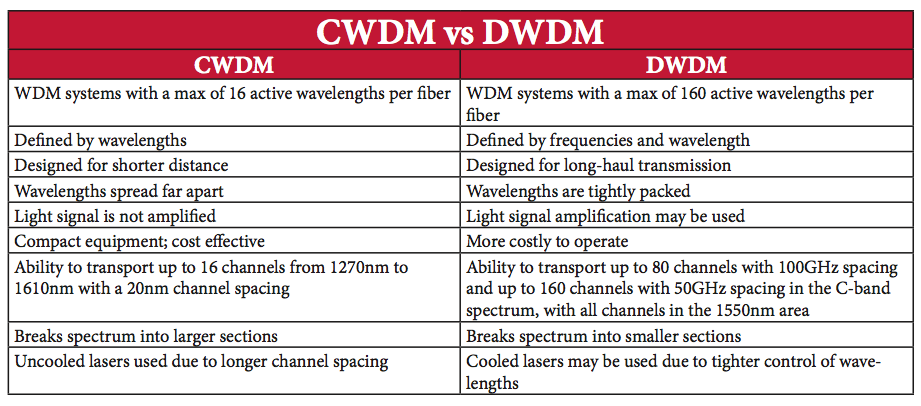
\includegraphics[width=12cm,height=8cm]{cwdm-vs-dwdm.png}
\caption[Comparison CWDM vs DWDM]{Comparison CWDM vs DWDM}
\label{Comparison CWDM vs DWDM}
\end{figure}
\section{Afocal Scheme}
\justify
In optics an afocal system (a system without focus) is an optical system that produces no net convergence or divergence of the beam, i.e. has an infinite effective focal length (theoretically). This type of system can be created with a pair of optical elements where the distance between the elements is equal to the sum of each element's focal length (d = f1+f2). \\
\\
Fig. 2.2.1 represents the afocal scheme, comprising two convex lenses with different focal lengths
of 10 cm (f1) and 5 cm (f2). 
\begin{figure}[H]
\centering
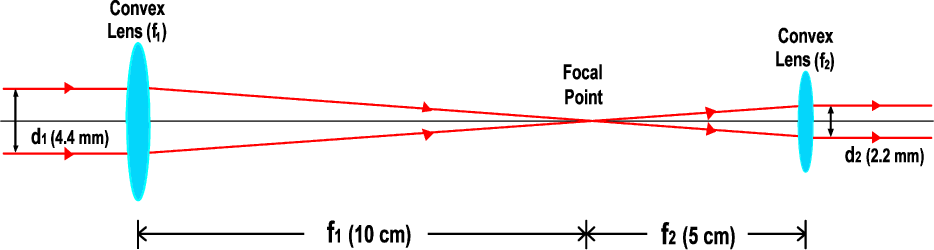
\includegraphics[width=12cm,height=4cm]{6-Figure4-1.png}
\caption[Afocal Scheme, with two convex lenses]{Afocal Scheme, with two convex lenses}
\label{Afocal Scheme, with two convex lenses}
\end{figure}

For this afocal scheme, the separation distance (d) of two convex
lenses is equal to the sum of the focal lengths (d = f1 + f2). The function of the afocal scheme
is to transform a collimated optical beam with a large diameter of 4.4 mm (d1) into another collimated
optical beam with a small diameter of 2.2 mm (d2).\\
\\
 If the afocal scheme is operated nearby the receiving site, then the afocal
scheme is the \textbf{pre-afocal scheme}. While if the afocal scheme is operated nearby the middle position,
then the afocal scheme is the \textbf{in-line afocal scheme}.\\
\\
\section{Bit Error Rate (BER)}
\justify
In digital transmission, the number of bit errors is the number of received bits of a data stream over a communication channel that have been altered due to noise, interference, distortion or bit synchronization errors.\\

\\The bit error rate (BER) is the number of bit errors per unit time. The bit error ratio (also BER) is the number of bit errors divided by the total number of transferred bits during a studied time interval. Bit error ratio is a unitless performance measure, often expressed as a percentage.\\

\\The bit error probability is the expectation value of the bit error ratio. The bit error ratio can be considered as an approximate estimate of the bit error probability. This estimate is accurate for a long time interval and a high number of bit errors.
The BER may be improved by choosing a strong signal strength (unless this causes cross-talk and more bit errors) or by choosing a slow and robust modulation scheme.
\section{Eye Pattern}
\justify
Eye pattern is a pattern displayed on the screen of a cathode ray oscilloscope (CRO) and is used as a tool for evaluating 
the effects of intersymbol interference (ISI).
The eye pattern derives its name from the fact 
that it resembles the shape of the human eye.
The interior region of the eye pattern is called 
eye opening. The eye pattern provides a great deal of information about the performance of the system.
\begin{itemize}
\item The width of the eye opening defines the time interval over which the received signal can be sampled without error from inter-symbol interference. The preferred time for sampling is the instant of time at which the eye is open the 
widest.
\item
The sensitivity of the system to timing errors is determined by the rate of closure of the eye as the sampling time is varied.
\item
The height of the eye opening defines the noise 
margin of the system.
\end{itemize}
Fig shows the interpretation of eye pattern:
\begin{figure}[H]
\centering
\includegraphics[width=10cm,height=8cm]{2018-09-09.png}
\caption[Interpretation of eye pattern]{Interpretation of eye pattern}
\label{Interpretation of eye pattern}
\end{figure}

\chapter{Experimental Setup}
Following figure depicts the experimental configuration of the proposed 50 m/320 Gbps DWDM FSO communications
that employs afocal scheme and DWDM technology.
\begin{figure}[H]
\centering
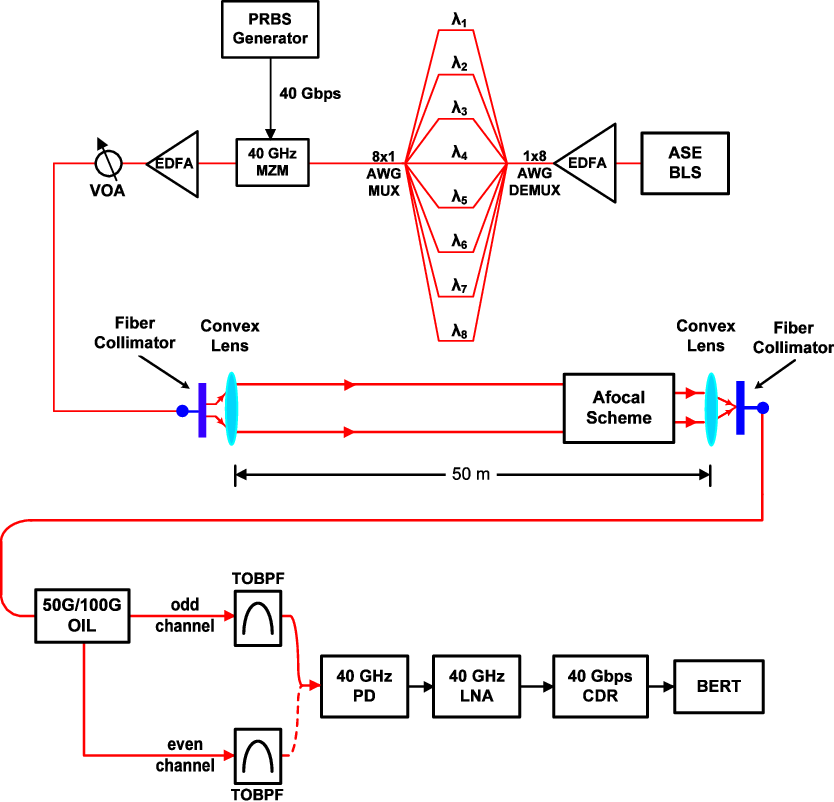
\includegraphics[width=10cm,height=8cm]{4-Figure1-1.png}
\caption[Experimental configuration of the proposed 50-m/320-Gb/s DWDM FSO communication that
employs afocal scheme and DWDM technology.]{Experimental configuration of the proposed 50-m/320-Gb/s DWDM FSO communication that
employs afocal scheme and DWDM technology.}
\label{Experimental configuration of the proposed 50-m/320-Gb/s DWDM FSO communication that
employs afocal scheme and DWDM technology.}
\end{figure}
\\
\section{Components of the experimental configuration}
\justify
Given below are the major components of the proposed experimental configuration.
\subsection{Amplified Spontaneous Emission (ASE) broadband light source (BLS)}
\justify
\textbf{Amplified spontaneous emission (ASE)} or superluminescence is light, produced by spontaneous emission, that has been optically amplified by the process of stimulated emission in a gain medium.\\
\\The gain medium (also called active laser medium or lasing medium) is the source of optical gain within a laser. The gain results from the stimulated emission of electronic or molecular transitions  (due to photons interacting with excited electrons) to a lower energy state from a higher energy state.\\
\\\textbf{A broadband light source} is a light source with a broad bandwidth, which does not necessarily emit in the visible spectral region. Such sources can be superluminescent sources, e.g. superluminescent diodes, and typically exhibit a high spatial coherence, making it easy to tightly focus the output or to deliver it through an optical fiber, even a single-mode fiber. 


\begin{figure}[H]
\centering
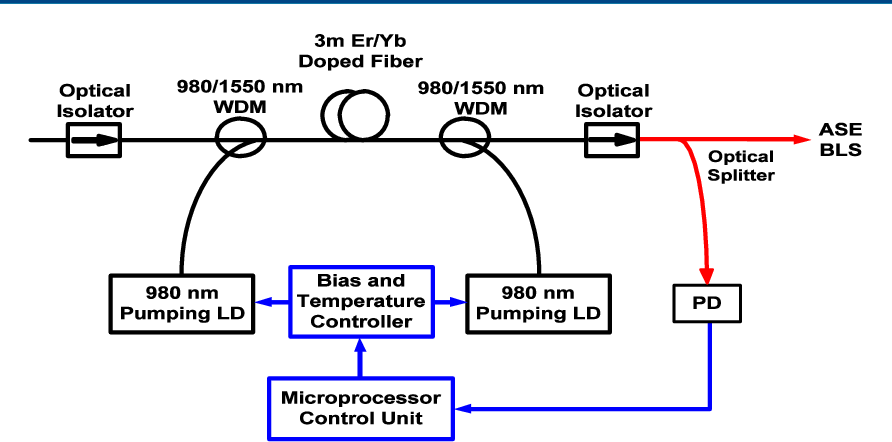
\includegraphics[width=10cm,height=5cm]{5-Figure2-1.png}
\caption[Configuration of the ASE BLS.]{Configuration of the ASE BLS.}
\label{Configuration of the ASE BLS.}
\end{figure}
\\
Fig. 3.1.1 shows the configuration of the ASE BLS, which is composed of a
bidirectional pumped erbium-doped
fiber amplifier (EDFA) with laser diodes (LDs) at 980 nm. Two 980 nm pumping laser diodes (LDs) with 180 mW pumping
power are coupled into a 3-m Er/Yb doped fiber by two 980/1550 nm WDM couplers. Two optical
isolators are used to prevent reflections which can degrade ASE BLS performance. Part of the
laser output is utilized for opto-electronic feedback to enhance the performance of ASE BLS, and
another part of the laser output is used for ASE BLS. A photodiode (PD) converts laser light into the electronic signal to control the microprocessor control unit and the bias and temperature controller.\\


\subsection{Erbium-Doped
Fiber Amplifier (EDFA)}
An optical amplifier is a device that amplifies an optical signal directly, without the need to first convert it to an electrical signal. Optical amplifiers are important in optical communication and laser physics. They are used as optical repeaters in the long distance fiberoptic cables which carry much of the world's telecommunication links. \\
\\Doped fiber amplifiers (DFAs) are optical amplifiers that use a doped optical fiber as a gain medium to amplify an optical signal. They are related to fiber lasers. The signal to be amplified and a pump laser are multiplexed into the doped fiber, and the signal is amplified through interaction with the doping ions.
\\The most common example is the Erbium Doped Fiber Amplifier (EDFA), where the core of a silica fiber is doped with trivalent erbium ions and can be efficiently pumped with a laser at a wavelength of 980 nm or 1,480 nm, and exhibits gain in the 1,550 nm region.
Fig 3.2.1 shows the schematic diagram of a simple EDFA:

\begin{figure}[H]
\centering
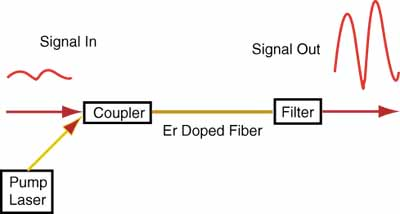
\includegraphics[width=10cm,height=5cm]{fa-diag.jpg}
\caption[schematic diagram of a simple EDFA]{schematic diagram of a simple EDFA}
\label{schematic diagram of a simple EDFA}
\end{figure}


\subsection{Arrayed Waveguide Grating (AWG) MUX and DEMUX}
\justify
AWG is used as optical multiplexer. This application is used in DWDM network to multiplex various WDM channels into one fiber cable.
They are also used as optical de-multiplexers at receiver end of DWDM network.
\subsection*{Operation of AWG}
\justify
For AWG to function as an optical demultiplexer, the following steps are followed.
\begin{figure}[H]
\centering
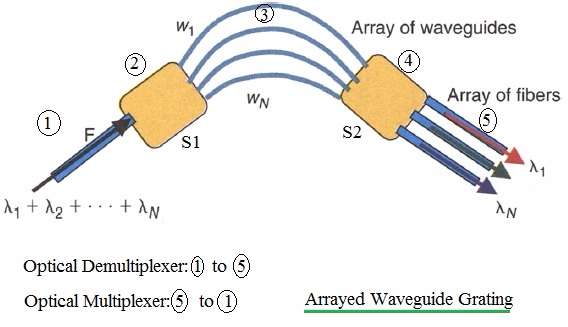
\includegraphics[width=10cm,height=6cm]{Arrayed-Waveguide-Grating-based-Optical-MUX-DEMUX.jpg}
\caption[Operation of AWG]{Operation of AWG}
\label{Operation of AWG}
\end{figure}
\begin{itemize}
    \item As shown in figure 3.3.1, incoming light signal having all wavelengths are fed using optical fiber(F) into input cavity or input coupler (designated as 'S1') part of the optical AWG.

\item This multiplexed signal is passed through the free space portion of 'S1'.

\item Next, light gets divided into array of waveguides. Here phase delay proportional to wavelength is introduced to optical signals passed from different waveguides of different lengths.

\item Now these phase delayed signals are made to pass from output cavity or output coupler (designated as 'S2') . This cavity is connected with multiple optical fiber cables. At this stage, light signals after passing through different lengths of waveguides will interfere with one another. As a result, each output optical fibers are fed with one unique wavelength of light having maximum amplitude.

\item At this stage, with the use of multiple optical fiber cables different wavelengths of light are taken as output.
\\ Fig 3.1.4 shows the optical spectrum of the sliced wavelengths.
\end{itemize}
\begin{figure}[H]
\centering
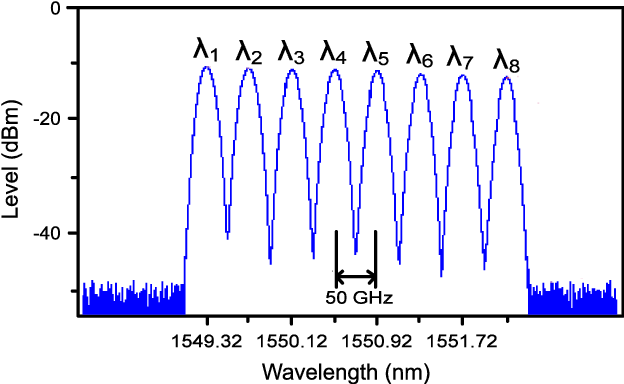
\includegraphics[width=10cm,height=6cm]{5-Figure3-1.png}
\caption[Optical Spectrum of the spectrum-sliced eight wavelengths]{Optical Spectrum of the spectrum-sliced eight wavelengths}
\label{Optical Spectrum of the spectrum-sliced eight wavelengths}
\end{figure}
 For AWG to be used as optical multiplexer reverse operations of the steps mentioned above will take place. Here individual light signals having different wavelengths are provided as input at location (5) of AWG and multiplexed output is derived from location (1) of AWG.


\subsection{Mach-Zehnder modulator (MZM)}
A Mach-Zehnder modulator is used for controlling the amplitude of an optical wave. It has a structure similar to a mach-zehnder interferometer (MZI), which is a device used to determine the relative phase shift variations between two collimated beams derived by splitting light from a single source. The interferometer has been used, among other things, to measure phase shifts between the two beams caused by a sample or a change in length of one of the paths. \\
\\ The input waveguide is split up into two waveguide interferometer arms. If a voltage is applied across one of the arms, a phase shift is induced for the wave passing through that arm. When the two arms are recombined, the phase difference between the two waves is converted to an amplitude modulation.\\
\begin{figure}[H]
\centering
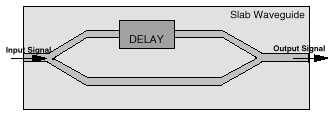
\includegraphics[width=10cm,height=6cm]{05-114.jpg}
\caption[MZM]{MZM}
\label{MZM}
\end{figure}
\\For example, if the phase shifts applied by the arms have a difference of 180 degrees, the output is zero and if no phase shift is applied, you can get the whole input in the output. Thus, amplitude modulation is possible.
\subsection{Variable Optical Attenuator (VOA)}
\justify
VOA is a device that can incrementally adjust the power of the optical signal passing through it.The power reduction is done by such means as absorption, reflection, diffusion, scattering, deflection, diffraction, and dispersion, etc.\\
\\Optical attenuators usually work by absorbing the light, like sunglasses absorb extra light energy. They typically have a working wavelength range in which they absorb all light energy equally. They should not reflect the light or scatter the light in an air gap, since that could cause unwanted back reflection in the fiber system.
\subsection{Fiber Collimators and Single Mode Fibers}
Collimated light is light whose rays are parallel, and therefore will spread minimally as it propagates. A perfectly collimated beam, with no divergence, would not disperse with distance.A collimator is a device that narrows a beam of particles or waves. To narrow means to cause the directions of motion to become more aligned in a specific direction i.e., make collimated light or parallel rays.
Fiber Collimators are devices for collimating the light coming from a fiber, or for launching collimated light into the fiber.\\
\\In fiber-optic communication, a single-mode optical fiber (SMF) is an optical fiber designed to carry light only directly down the fiber - the transverse mode. Modes define the way the wave travels through space, i.e. how the wave is distributed in space. Waves can have the same mode but have different frequencies. This is the case in single-mode fibers, where we can have waves with different frequencies, but of the same mode, which means that they are distributed in space in the same way, and that gives us a single ray of light. 
\begin{figure}[H]
\centering
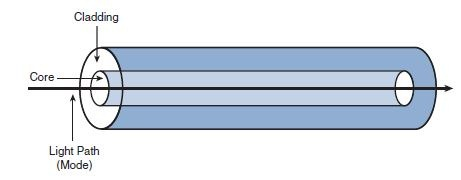
\includegraphics[width=10cm,height=4cm]{single-mode-fiber.jpg}
\caption[The structure of a typical single-mode fiber.
]{The structure of a typical single-mode fiber.
}
\label{The structure of a typical single-mode fiber.}
\end{figure}
\subsection{Optical Interleaver (OIL)}
\justify
An optical interleaver is a 3-port passive fiber-optic device that is used to combine two sets of dense wavelength-division multiplexing (DWDM) channels (odd and even channels) into a composite signal stream in an interleaving way. For example, optical interleaver takes two multiplexed signals with 100 GHz spacing and interleaves them, creating a denser DWDM signal with channels spaced 50 GHz apart. 
\\The device can be used in a reverse direction, forming an optical deinterleaver that separates a denser DWDM signal into odd channels and even channels, as shown in figure 3.7.1.
\begin{figure}[H]
\centering
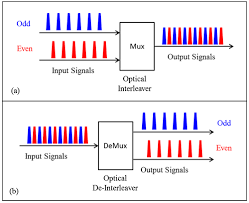
\includegraphics[width=10cm,height=4cm]{index.png}
\caption[An Optical Interleaver]{An Optical Interleaver}
\label{An Optical Interleaver}
\end{figure}
\subsection{Tunable Optical Band Pass Filter (TOBPF)}
A Tunable optical filter is ideal for any application requiring wavelength tuning, such as
\begin{itemize}
    \item Optical Channel Performance Monitoring
    \item Optical Signal Noise Suppression
    \item Optical Signal Tracking 
\end{itemize}
A TOBPF is a band pass filter and can pass any frequency required. It is tunable meaning it can be tuned to pass a certain frequency component over other components.
\begin{figure}[H]
\centering
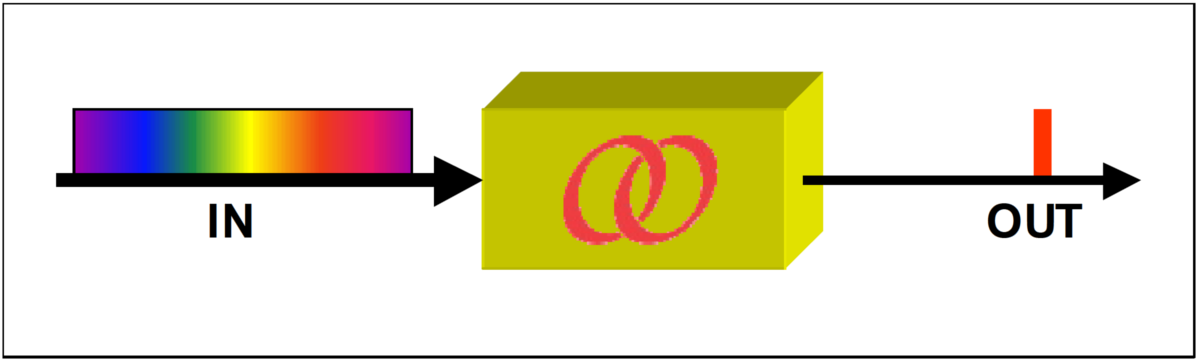
\includegraphics[width=10cm,height=4cm]{MEMS-TF-1.png}
\caption[Tunable Optical Band Pass Filter ]{Tunable Optical Band Pass Filter }
\label{Tunable Optical Band Pass Filter }
\end{figure}
\subsection{Low Noise Amplifier (LNA)}
\justify
 Low-noise amplifier (LNA) is an electronic amplifier that amplifies a very low-power signal without significantly degrading its signal-to-noise ratio. An amplifier increases the power of both the signal and the noise present at its input. LNAs are designed to minimize additional noise. \\
 \\ Typical LNA may supply a power gain of 100 (20 decibels (dB)) while decreasing the signal-to-noise ratio by less than a factor of two (a 3 dB noise figure (NF)).The noise figure helps determine the efficiency of a particular LNA. LNA suitability for a particular application is typically based on its noise figure. In general, a low noise figure results in better signal reception. 
 \subsection{Clock and Data Recovery (CDR)}
 \justify
 Since most of the high speed serial interfaces do not have any accompanying clock, the receiver needs to recover the clock in order to sample the data on serial lines.\\
\\
To recover the sampling clock, receiver needs a reference a clock of approximately same frequency. To generate the recovered clock, the receiver needs to phase align the reference clock to the transitions on the incoming data stream. This is called as Clock recovery.\\

\\Sampling of that incoming data signal with recovered clock to generate a bit stream is called as Data recovery. Together, this is called Clock Data Recovery, or CDR.\\

\\CDR is required to recover data from incoming data stream in the absence of any accompanying clock signal, without any bit errors due to over/under sampling.
\begin{figure}[H]
\centering
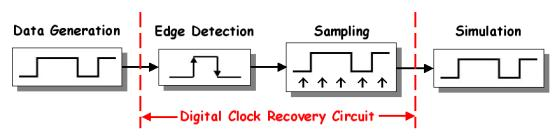
\includegraphics[width=10cm,height=4cm]{block_diagram.jpg}
\caption[CDR  ]{CDR }
\label{CDR  }
\end{figure}
\subsection{Bit Error Rate Tester (BERT)}
\justify
Bit error rate, BER testing and bit error rate testers are used for testing systems that transmit digital data from one location to another. When data is transmitted there is a possibility of errors being introduced into the system, especially if the medium over which the data is transmitted is noisy. If errors are introduced into the data, then the integrity of the system may be compromised. As a result a bit error rate test can indicate much about the link quality and the ability of the system to accommodate the link characteristics.\\
\begin{figure}[H]
\centering
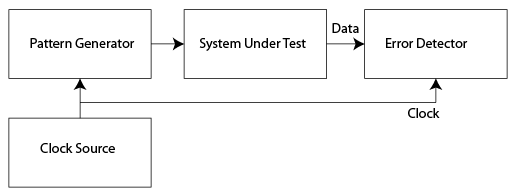
\includegraphics[width=10cm,height=4cm]{image57.png}
\caption[BERT block diagram  ]{BERT block diagram }
\label{BERT block diagram  }
\end{figure}
\\A data stream is sent through the communications channel, whether a radio link or a fibre optic link, and the resulting data stream is compared with the original. Any changes are noted as data errors and logged. Using this information a bit error rate can be determined.\\
\\A BER test provides a measurable and useful indication of the performance of the performance of the system that can be directly related to its operational performance. If the BER rises too high then the system performance will noticeably degrade. If it is within limits then the system will operate satisfactorily.
\section{Experimental procedure}
The output of the amplified
spontaneous emission (ASE) broadband light source (BLS) is amplified by an erbium-doped
fiber amplifier (EDFA) and efficiently split into eight optical channels by a 1 x 8 arrayed waveguide
grating (AWG) demultiplexer (DEMUX) with a channel spacing of 0.4 nm (50 GHz). Eight
wavelengths from the AWG DEMUX output are multiplexed into a 40-GHz Mach–
Zehnder modulator (MZM) by a 8 x 1 AWG multiplexer (MUX). The MZM is modulated by a
40-Gbps pseudorandom binary sequence (PRBS) generated by a PRBS generator. It
means that the same PRBS sequence is transmitted over all eight channels. \\
\\A variable optical
attenuator (VOA) is positioned at the start of the second-stage EDFA so that the optical power
launched into the free-space can be optimized to obtain the best transmission performances.
Given that EDFA can only amplify optical signals in the 1550 nm region, thereby, such DWDM
FSO communications are enhanced by the introduction of 1550 nm technology. A pair of fiber
collimators is used to collimate light from a fiber to form a collimated optical beam and to guide a
collimated optical beam from the free-space into an optical fiber. The fiber collimators connected
to single-mode fibers (SMFs) play an important role in forming an optical beam to transport optical
signal through the free-space between the two sides. This fiber collimator has an operating
wavelength range of 1050–1620 nm, a fiber-to-lens distance of 7.5 mm, and a focal length of
7.5 mm. The light emitted from the first-stage fiber collimator is launched into the first-stage
convex lens, delivered in the free-space, inputted into an afocal scheme, and fed into the
second-stage convex lens to concentrate on the second-stage fiber collimator.The function of
the first-stage convex lens is to transform the divergent beam into the parallel beam, the function
of the afocal scheme is to reduce the beam size of the collimated optical beam, and the function
of the second-stage convex lens focusses the reduced parallel beam into a point.\\
\\Over a 50-m free-space link, the eight laser lights with a total data stream of 320 Gbpsreached to a 50G/100G optical interleaver (OIL). An OIL is deployed at the
receiving site to separate odd and even optical sidebands of the optical signal. The OIL has two
output ports; one output port provides the optical signal only with the odd optical sidebands, and
the other output port provides the optical signal only with the even optical sidebands. The OIL
used in this experiment has an input channel spacing of 50 GHz and an output channel spacing
of 100 GHz. Following the OIL output with odd (even) optical sidebands, the optical sidebands
are separated by a spacing of 100 GHz and fed into a tunable optical band-pass filter (TOBPF),with a 3-dB bandwidth of 0.32 nm, to select the desired wavelength. \\
\\The selected optical wavelength
is then detected by a 40-GHz photodiode (PD) with a responsivity of 0.55 mA/mW (at
1550 nm) and amplified by a 40-GHz Low Noise Amplifier(LNA) with a small signal gain of 20 dB (measured at
40 GHz) and a noise figure of around 2 dB. It is necessary for an LNA to amplify the data stream
while adding as little noise and distortion as possible. After LNA amplification, the data stream is
recovered and regenerated by a 40-Gbps Clock and Data Recovery Circuit (CDR) and fed into a bit error rate tester (BERT) for
BER performance analysis. The function of the CDR is to recover and regenerate the data
stream from the distorted data stream. Considering that BER will increase as the receiver cannot
discriminate between noise and transmitted data, a CDR is necessary at the receiving site.
\chapter{Experimental Results and Discussion}
The following results were obtained from the experiment:
\begin{itemize}
    \item At a free-space transmission distance of 50 m, as LNA and CDR are
not employed, the BER is approximately 10-5. However, as LNA and CDR are employed simultaneously,
the BER reaches around  10-9.
Fig  shows the measured BER curves of DWDM FSO communications at a data stream of 40 Gbps.
\begin{figure}[H]
\centering
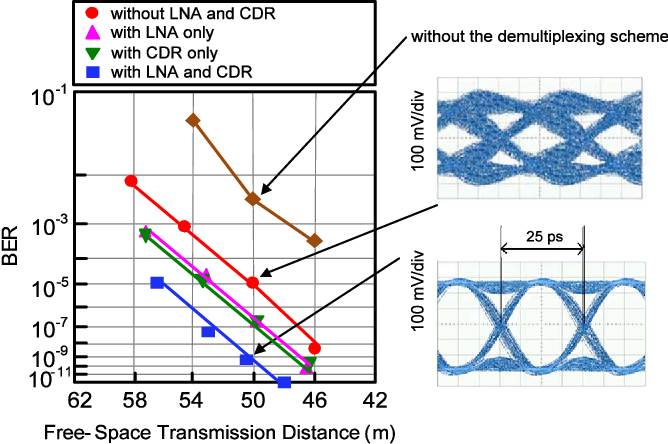
\includegraphics[width=10cm,height=6cm]{7-Figure5-1.png}
\caption[Measured BER curves of DWDM FSO communication at a data stream of 40 Gb/s ]{Measured BER curves of DWDM FSO communication at a data stream of 40 Gb/s }
\label{Measured BER curves of DWDM FSO communication at a data stream of 40 Gb/s }
\end{figure}
\item To better show the relation with LNA, CDR, and
BER performance, one of the BER performance improvement schemes is removed. Clearly,
when only one BER performance improvement scheme is employed, the BER performance improvement
is restricted. 
\item Fig. 4.0.1 also shows the eye diagrams
of the 40 Gbps data stream  over a 50-m free-space link with/without employing LNA
and CDR. Amplitude and phase fluctuations are obviously observed when LNA and CDR are
not employed. As LNA and CDR are employed simultaneously, however, a clear eye diagram is
observed due to the suppression of amplitude and phase fluctuations.
\item To show a direct association
with the demultiplexing scheme and the BER performance, the demultiplexing
scheme (without employing OIL and TOBPF at the receiving site) is removed and  the BER performance is evaluated,
as LNA and CDR are employed concurrently. It can be seen that a serious BER performance degradation exists due to crosstalk and interference from other wavelengths.
\begin{figure}[H]
\centering
\includegraphics[width=8cm,height=8cm]{aaa.png}
\caption[Measured BER curves of DWDM FSO communication at a data stream of 40 Gb/s  over
46-m/50-m/54-m/58-m free-space transmission distances as LNA and CDR are employed
concurrently. ]{Measured BER curves of DWDM FSO communication at a data stream of 40 Gb/s  over
46-m/50-m/54-m/58-m free-space transmission distances as LNA and CDR are employed
concurrently. }
\label{Measured BER curves of DWDM FSO communication at a data stream of 40 Gb/s  over
46-m/50-m/54-m/58-m free-space transmission distances as LNA and CDR are employed
concurrently. }
\end{figure}
\item Fig. 4.0.2 shows the measured BER curves of DWDM FSO communications at a data stream of
40 Gbps  over 46 m/50 m/54 m/58 m free-space transmission distances, as LNA and CDR
are employed concurrently. As shown, as the free-space transmission distance increases the
BER value increases as well. As the free-space transmission distance is larger than 50 m, the
BER value is higher than 10-9.
\end{itemize}

\section{Discussion}
The following inferences can be made from the experiment:
\begin{itemize}
    \item Excellent BER performance is obtained to demonstrate the possibility of establishing a
50 m/320 Gbps DWDM FSO communication. Both of the LNA and CDR play important roles for BER improvement.
They can improve the error vector magnitude (EVM) and signal-to-noise ratio (SNR) values of
FSO communications, leading to BER performance improvement.
\item If there
is no demultiplexing scheme at the receiving site, then the crosstalk and channel interference
that arise from other wavelengths will increase significantly. The
demultiplexing scheme must reject the adjacent channels so that they do not interfere. 
\item Longer free-space transmission distance results in lower received
optical power, by which leading to the deterioration of BER performance. The free-space
transmission distance can be extended not only by the optimization of the afocal scheme, but
also by the employment of an EDFA with higher optical output power. By employing an EDFA
with higher optical output power, higher optical power can be launched into the free-space to
compensate for the loss of the link. A trade-off occurs between the transmission distance and
the transmission rate. Error-free operation can be achieved under different transmission distances
with different transmission rates.
\end{itemize}
The following are the challenges faced by the present experimental setup:
\begin{itemize}
    \item The simplification of the BLS is a key issue that should be addressed in the development of DWDM
FSO communications.
\begin{itemize}
    \item A BLS, comprising optoelectronic oscillator (OEO) and optical signal-to noise
ratio (OSNR) enhancement schemes, has been demonstrated previously. However,
sophisticated OEO and OSNR enhancement schemes are required.
\item High power superluminescent
diodes (SLDs)-based BLS has been illustrated previously. Nonetheless, it is not
flexible due to a narrow optical 3-dB bandwidth.
\end{itemize}    
Spectrum slicing is a feasible technique by which
narrow wavelengths are filtered from a BLS and externally modulated to deliver optical signals. 
\item To guarantee a successful implementation of a DWDM FSO communication,
the wavelengths are selected from the odd
(even) channel output of the OIL to prevent the crosstalk that arises from the incomplete isolation
of the adjacent channels. If only a TOBPF is employed for the demultiplexing (without employing
OIL at the receiving site), then the crosstalk that arises from the incomplete isolation of the adjacent
channels will obviously increase due to a close channel spacing of 50 GHz. And such crosstalk increment
will result in the degradation of BER performance. The function of the demultiplexing
scheme is to distinguish each optical wavelength without crosstalk and channel interference. It is a
great challenge in closely spaced optical wavelengths.
\item As the free-space transmission distance
increases, the received OSNR decreases because other lights form the
environment are also received by the PD. Noise is generated when other lights form the environment
are received by the PD. As the free-space transmission distance increases the noise
increases as well, by which resulting in the decrement of OSNR value and the degradation of
BER performance. Thereby, there is a trade-off between the free-space transmission distance
(the focal length ratio) and the BER performance. To guarantee a successful design of FSO
communication, system designers will have to address the optimization of the afocal scheme
(the optimum focal length ratio of the afocal scheme).
\item The FSO communication is to realize the free-space transmission using a pair of fiber collimators
with SMFs. Propagating an optical beam through the free-space between the fiber collimators
enacts the FSO communication to work as if the fibers were connected seamlessly. Optical
beam alignment and focal spot size between convex lens and fiber collimator are critical for the
transmission performance of an FSO communication. An FSO communication with optical beam
misalignment and divergent focal spot size (the focal spot size greater than the mode field size of the fiber)
between convex lens and fiber collimator will degrade the transmission performance.
\end{itemize}




%\addcontentsline{toc}{chapter{Conclusion and future scope}}
\chapter{Conclusion and future scope}
\justify
Applications of DWDM and Afocal Scheme in Free Space Optics is a promising and rapidly progressing research avenue in modern optics. A DWDM FSO communication that adopts afocal scheme and DWDM technology is proposed.
The free-space transmission distance and transmission rate are greatly increased by afocal
scheme and DWDM technology. A total transmission rate of 320 Gbps is successfully delivered
over a 50-m free-space link. The proposed DWDM FSO communications are experimentally
demonstrated with low BER operation and clear eye diagram. The findings demonstrated that
such a DWDM FSO communication can provide the advantages of optical wireless links for long
transmission distance and high transmission rate. With more advancements in FSO, it can replace OFCs in telecommunication applications.\\
\pagebreak

\addcontentsline{toc}{chapter}{Bibliography}
\begin{thebibliography}{1}
\bibitem{ib} W. S. Tsai et al., “A 50-m/320-Gb/s DWDM FSO Communication With Afocal Scheme”, \textit{IEEE Photon. J.,} vol. 8, no. 3, June 2016, Art. No. 2555618.

\bibitem{ib} W. S. Tsai et al., “A 20-m/40-Gb/s 1550-nm DFB LD-based FSO link,” \textit{IEEE Photon. J.,} vol. 7, no. 6, Dec. 2015,
Art. no. 7905907.
 
\bibitem{em}H. Henniger and O. Wilfert, “An introduction to free-space optical communications,” \textit{Radioen.,} vol. 19, no. 2,
pp. 203–212, Jun. 2010.
\bibitem{band}W. S. Tsai et al., “A 50 m/40 Gbps 680-nm VCSEL-based FSO communication,” \textit{IEEE Photon. J., }vol. 8, no. 2,
Apr. 2016, Art. no. 7903008.


\bibitem{photon} J. Yu et al., “DWDM optical millimeter-wave generation for radio-over-fiber using an optical phase modulator and an
optical interleaver,” IEEE Photon. Technol. Lett., vol. 18, no. 13, pp. 1418–1420, Jul. 2006.


\bibitem{effect} H. H. Lu et al., “Bidirectional fiber-wireless and fiber-VLLC transmission system based on an OEO-based BLS and a
RSOA,” \textit{Opt. Lett., }vol. 41, no. 3, pp. 476–479, Feb. 2016.

\bibitem{}G. A. Alphonse, D. B. Gilbert, M. G. Harvey, and M. Ettenberg, “High-power superluminescent diodes,” \textit{IEEE J.
Quantum Electron.,} vol. 24, no. 12, pp. 2454–2457, Dec. 1988.




\end{thebibliography}
\end{document}
